\chapter{Background}

\section{Introduzione al DNS e al filtraggio}
Prima di trattare l'argomento cardine del presente capitolo, si ritiene opportuno fare una breve panoramica sui concetti importanti ad esso collegati. Verrà in prima batttuta presentato il Domain Name System (DNS), che può essere definito come uno dei pilastri fondamentali di tutta l'architettura della rete Internet. Successivamente, ci si sposterà sull'ambito del filtraggio in Internet, che rappresenta il contesto più ampio di cui il filtraggio DNS fa parte.

\subsection{Cos'è il DNS e il suo ruolo in Internet}
Il Domain Name System è un database gerarchico e distribuito che contiene le associazioni tra nomi di dominio ed altre importanti informazioni, tra cui gli indirizzi IP.

Questo fondamentale sistema consente agli utenti di localizzare le risorse sulla rete andando a convertire nomi di dominio familiari ed in formato leggibile dagli umani in indirizzi numerici ai quali un computer può connettersi. Un'analogia comune che si uutilizza per spiegare il ruolo dei sistema DNS è che esso serve da rubrica telefonica per Internet, andando a tradurre i nomi di computer comprensibili agli umani nei relativi indirizzi numerici interpretabili dalle macchine. Per fare un esempio, il nome di dominio \texttt{www.airbus.com} viene tradotto dal DNS nell'indirizzo IPv4 \texttt{107.154.76.155}.

\subsubsection{Vulnerabilità del DNS}
Il DNS rappresenta una porzione cruciale della rete Internet e per questo motivo la sua messa in sicurezza risulta molto importante. Infatti, se un individuo malintenzionato dovesse riuscire a comprometterlo, sarebbe in grado di bloccare, o comunque ridurre, le normali attività che avvengono sulla rete.

Il sistema in oggetto è stato progettato negli anni '80 per rispondere alla necessità di una risoluzione dei nomi rapida e scalabile su una rete in continua espansione. Al momento della sua concezione, come descritto nelle specifiche originarie RFC 1034 \cite{DBLP:journals/rfc/rfc1034} e RFC 1035 \cite{DBLP:journals/rfc/rfc1035}, l'attenzione era principalmente concentrata sulla funzionalità e sull'efficienza, senza considerare i potenziali problemi di sicurezza che sarebbero emersi con la crescita esponenziale di Internet. Oltretutto, la solida fiducia che le specifiche RFC trasmettevano ai professionisti IT dell’epoca li ha portati a trascurare o a non approfondire i potenziali rischi di sicurezza associati a tale sistema \cite{hudaib2014dns}. Questa scelta rifletteva il contesto storico in cui è nato il DNS: la rete era allora utilizzata principalmente da enti accademici e governativi, con un livello di fiducia reciproca tra i partecipanti. Tuttavia, con l'apertura di Internet a un pubblico globale, il DNS ha rivelato vulnerabilità intrinseche, tra cui la mancanza di meccanismi nativi che garantiscano l'autenticazione delle risposte e l'integrità delle informazioni da esso fornite. Tali lacune hanno reso possibile una serie di attacchi che sfruttano le debolezze intrinseche del sistema DNS. Tra questi, figurano il DNS Spoofing, il DNS Amplification Attack e il DNS Hijacking.

\paragraph{DNS Spoofing}\label{paragraph:dns_spoofing}
Il DNS spoofing, noto anche come Cache Poisoning, consiste nell'iniettare dati malevoli nella cache dei server DNS bersaglio, inducendoli a restituire informazioni errate agli utenti. Questo attacco permette ai malintenzionati di reindirizzare il traffico verso siti controllati da essi, facilitando il furto di credenziali o altre forme di attacchi avanzati. Un esempio storico di DNS spoofing è l'attacco di Eugene Kashpureff del 1997, il quale riuscì a reindirizzare tutti i visitatori del dominio \texttt{internic.net} verso il sito della compagnia Alternic, di cui era il fondatore \cite{lioy2000dns}.

In generale, questa tipologia di attacco sfrutta la mancanza di autenticazione nelle risposte DNS e l'assenza di integrità nelle informazioni memorizzate nella cache. I metodi per mitigare il DNS spoofing includono sostanzialmente l'implementazione di DNSSEC, che garantisce l'autenticità delle risposte attraverso firme digitali \cite{DBLP:journals/rfc/rfc2535}.

\paragraph{DNS Amplification Attacks}
Gli attacchi di tipo Distributed Denial of Service (DDoS) rappresentano una delle minacce più critiche per la sicurezza informatica, mirate a compromettere la disponibilità di un sistema. Questi attacchi si basano sull'invio massivo di richieste a un bersaglio per esaurirne le risorse, come CPU, memoria o larghezza di banda, rendendo il servizio inaccessibile agli utenti legittimi.

Un esempio rilevante nell'ambito del DNS è rappresentato dagli attacchi di amplificazione, una tipologia particolarmente efficace di DDoS. In questi attacchi, l'aggressore invia richieste DNS utilizzando un indirizzo IP sorgente falsificato, facendole sembrare provenienti dalla vittima. I server DNS, ingannati, rispondono con pacchetti significativamente più grandi delle richieste originali, amplificando così il volume del traffico diretto alla vittima. Sfruttando la differenza tra la dimensione delle richieste e delle risposte, gli attaccanti sono in grado di moltiplicare il traffico generato, saturando rapidamente le risorse della vittima e compromettendone il funzionamento \cite{DBLP:conf/ictc/AlieyanKARA16}.

Per difendersi dagli attacchi di amplificazione DNS, i fornitori di servizi Internet possono limitare l'accesso al proprio server DNS solamente agli utenti autorizzati, monitorare il traffico in entrata per individuare anomalie, e impostare dei limiti alla quantità di dati che il server DNS può inviare in risposta a una query.

Un caso pratico di amplificazione DNS è quello che ha colpito Spamhaus nel 2013, considerato uno dei più grandi attacchi DDoS mai accaduti. Esso è stato caratterizzato da una richiesta di 36 byte che ha generato una risposta di 3.000 byte, amplificando il traffico di un fattore 100 e generando un volume di dati in entrata ai server della compagnia pari a 75GBps \cite{Bonasera2021}.

\paragraph{DNS Hijacking}
Il DNS hijacking prevede la compromissione di server DNS o la manipolazione delle configurazioni DNS di un utente per reindirizzare il traffico verso destinazioni controllate da un malintenzionato. Questo tipo di attacco può essere implementato seguendo due strategie \cite{hudaib2014dns}:
\begin{itemize}
  \item attraverso l'uso di specifici malware che modificano le impostazioni DNS locali, oppure
  \item mediante la compromissione diretta dei server DNS fidati, in modo che non si comportino come da specifica.
\end{itemize}

Le conseguenze di questo tipo di attacco includono il furto di credenziali, la diffusione di malware e la censura di contenuti web. Tuttavia, alcuni provider di servizi Internet (ISP) utilizzano questa tecnica per scopi commerciali, come la visualizzazione di pubblicità o la raccolta di statistiche sulla navigazione dei propri clienti. Per mitigare il DNS hijacking, si consiglia di utilizzare configurazioni DNS sicure e controllare in maniera scrupolosa le modifiche ai record DNS locali \cite{hudaib2014dns}.

\subsection{Il filtraggio di Internet}
A seguito dell'analisi riguardante le vulnerabilità intrinseche del sistema DNS, emerge chiaramente l'importanza di adottare meccanismi di prevenzione per garantire una navigazione più sicura e controllata. A questo proposito, una soluzione interessante riguarda il filtraggio di Internet, che, in generale, rappresenta un insieme di tecniche e tecnologie volte a limitare o bloccare l'accesso a contenuti considerati inappropriati, illegali o dannosi. Le principali pratiche di filtraggio nell'ambito di Internet si dividono nelle tre seguenti tipologie:
\begin{itemize}
  \item \textbf{IP Packet Filtering}: ovvero il blocco del traffico basato su indirizzi IP o numeri di porta. Questa tecnica analizza gli header dei pacchetti per decidere se consentirne il passaggio o eliminarli. Sebbene sia semplice ed efficiente, può causare sovrafiltraggio, rendendo inaccessibili tutti quei contenuti legittimi ospitati su un indirizzo IP considerato malevolo;

  \item \textbf{DNS Poisoning}: consiste nella manipolazione delle risposte DNS per reindirizzare richieste a indirizzi errati o per bloccarle completamente. Sebbene sia nata come una pratica malevola (\Cref{paragraph:dns_spoofing}), i suoi principi tecnici sono stati adattati ed applicati ad un contesto legittimo di filtraggio;

  \item \textbf{URL Blocking}: implementa il blocco di URL specifici tramite proxy HTTP o tecniche come la Deep Packet Inspection (DPI). Questi sistemi analizzano il contenuto delle richieste HTTP per identificare e bloccare pagine o risorse specifiche, offrendo una maggiore precisione rispetto ai metodi sopra elencati. L'unico svantaggio di quest'ultimo approccio deriva dal fatto che risulta più complesse da implementare e richiede una maggiore potenza di calcolo rispetto alle altre tecniche.
\end{itemize}

\subsubsection{Punti di applicazione del filtraggio di Internet}
Il filtraggio di Internet può essere implementato in diversi livelli dell'architettura di rete, con implicazioni specifiche in termini di efficacia, costi e complessità. Secondo V. Varadharajan \cite{DBLP:journals/ieeesp/Varadharajan10}, i principali punti di applicazione includono:

\begin{itemize}
  \item \textbf{A monte dell'ISP}: i filtri possono essere posizionati nei fornitori internazionali di connettività o presso le dorsali di rete. Questo approccio consente di bloccare contenuti indesiderati prima che raggiungano l'ISP locale, risultando particolarmente utile per gestire il traffico proveniente da server internazionali. Tuttavia, questa strategia richiede una stretta collaborazione tra le entità coinvolte e una chiara mappatura dei gateway internazionali.

  \item \textbf{All'interno dell'ISP}: posizionare i filtri nel cuore della rete dell'ISP permette di monitorare e controllare il traffico a livello centralizzato per tutti i suoi utenti. Sebbene sia efficace, questa soluzione può introdurre colli di bottiglia e richiedere investimenti significativi in hardware sofisticato, soprattutto per ISP con un alto volume di traffico.

  \item \textbf{Tra l'ISP e il cliente}: applicare il filtraggio nel collegamento tra l'ISP e il cliente finale offre un controllo mirato sul traffico diretto verso reti locali o singoli utenti. Questa configurazione consente di personalizzare le policy di filtraggio in maniera più granulare rispetto ai precedenti punti di applicazione, ma può comportare costi operativi elevati per ISP con grandi numeri di clienti.

  \item \textbf{Tra due clienti dello stesso ISP}: in reti locali o interne a un ISP, i filtri possono essere configurati per impedire lo scambio di contenuti indesiderati tra utenti dello stesso provider. Questo approccio è utile in contesti aziendali o comunità chiuse.

  \item \textbf{Tra un cliente e un sito web ospitato a livello internazionale}: i filtri possono essere utilizzati per monitorare e bloccare il traffico tra un utente e server situati all'estero. Questa strategia è fondamentale per controllare contenuti provenienti da altri paesi, ma richiede un'infrastruttura adeguata e la capacità di gestire connessioni internazionali.
\end{itemize}

La possibilità di distribuire le tecniche di filtraggio su diversi livelli offre un'elevata flessibilità nell'implementazione delle strategie di controllo dei contenuti. Tuttavia, ogni livello si porta con sé alcuni compromessi: il posizionamento a monte può bloccare grandi volumi di traffico, ma con rischi di sovrafiltraggio, mentre i filtri localizzati vicino agli utenti offrono maggiore precisione ma richiedono risorse significative. Una combinazione di approcci, come quella messa in atto dalla British Telecom’s CleanFeed, può ottimizzare l'efficacia del filtraggio, bilanciando precisione e scalabilità \cite{DBLP:journals/ieeesp/Varadharajan10}.

\subsection{Il filtraggio DNS}
Tra le varie tecniche di Internet filtering descritte in precedenza, il filtraggio a livello DNS si distingue per la sua semplicità e versatilità. Al contrario di altri approcci, esso agisce direttamente sul sistema che costituisce la base della navigazione online. Questo lo rende un punto di controllo strategico ed efficace per implementare politiche di sicurezza e controllo dell'accesso. Oltretutto, i cybercriminali stanno sempre di più prendendo di mira l'infrastruttura DNS per condurre le loro attività malevole. Per questo motivo, le tecniche di filtraggio a questo livello assumono un ruolo centrale nella missione di rendere la rete più sicura e proteggere gli utenti dai rischi di attacchi. Nei paragrafi successivi verrà fornita una definizione del metodo in questione, insieme a dettagli sulle sue applicazioni pratiche e sulle modalità che ne abilitano il funzionamento.

Il \textit{DNS Filtering} consiste nell'applicare regole predefinite per bloccare o consentire richieste e risposte DNS, analogamente a quello che fa un firewall. Questa tecnica è in grado di prevenire l'accesso a contenuti malevoli o inappropriati, supportare l'applicazione di politiche aziendali e proteggere gli utenti da minacce provenienti dalla rete \cite{DBLP:journals/corr/abs-2401-03864}. Volendo essere più specifici, il filtraggio DNS trova applicazione in una vasta gamma di scenari pratici \cite{Murdoch2008,DBLP:journals/ieeesp/Varadharajan10}:
\begin{itemize}
  \item \textbf{Sicurezza informatica}: viene utilizzato per bloccare siti di phishing o che distribuiscono malware e altri contenuti dannosi;

  \item \textbf{Applicazione di politiche aziendali}: permette alle organizzazioni di imporre restrizioni sull'accesso a siti non correlati al lavoro, come social media o piattaforme di streaming, durante l'orario lavorativo;

  \item \textbf{Controllo parentale}: consente la creazione di un ambiente sicuro per i minori, limitando l'accesso a contenuti non appropriati come siti per adulti o violenti;

  \item \textbf{Gestione della larghezza di banda}: aiuta a limitare l'accesso a siti che consumano molta banda, come i servizi di streaming video, ottimizzando così l'utilizzo delle risorse di rete.
\end{itemize}

Dopo aver introdotto il concetto di filtraggio DNS e averne illustrato le principali applicazioni pratiche, è importante approfondire le tecniche utilizzate per la sua implementazione. Sebbene il DNS Filtering sia ampiamente riconosciuto come uno strumento fondamentale per migliorare la sicurezza delle reti, la sua efficacia dipende dall'applicazione di metodi avanzati per identificare e bloccare le minacce. Come evidenziato in letteratura, la ricerca ha individuato tre tecniche principali che rappresentano lo stato dell'arte in questo campo, ovvero le \textit{Response Policy Zones} (RPZ), i \textit{Threat Intelligence Feeds} (TIF) e il rilevamento di domini generati algoritmicamente (\textit{Domain Generation Algorithm}, DGA) \cite{DBLP:journals/corr/abs-2401-03864}.

Queste tecniche non solo permettono di affrontare le minacce più comuni, come phishing e malware, ma forniscono anche strumenti per rispondere a sfide più complesse, come il rilevamento di domini dinamici utilizzati per comunicare con le botnet. Tuttavia, la letteratura sottolinea anche alcune lacune, in particolare la mancanza di un'analisi integrata di queste metodologie. Approfondire ciascuna di esse consente di comprendere meglio il loro funzionamento, le applicazioni e i limiti, fornendo una base solida per ulteriori miglioramenti nel campo del DNS Filtering. A questo proposito, le sezioni seguenti saranno dedicate all'approfondimento delle tecniche appena citate, per poi fornire uno spunto su come potrebbero essere unite insieme per migliorare significativamente le performance del filtri.

\subsubsection{Response Policy Zones}
L'espressione Response Policy Zones descrive una funzionalità dei resolver DNS che consente agli amminsitratori di rete di specificare politiche per le risposte DNS, sulla base dei nomi di dominio e del contesto. Questa tecnologia opera intercettando le query e le risposte DNS, per poi confrontarle con un elenco di politiche definite dall'amministratore. Quando viene rilevata una corrispondenza, il resolver restituisce una risposta in base alla politica, che poi rappresenta l'azione da compiere. Esempi di possibili azioni, sono bloccare una certa query oppure reindirizzarla verso un sito sicuro (\Cref{fig:rpz}).

\begin{figure}
  \centering
  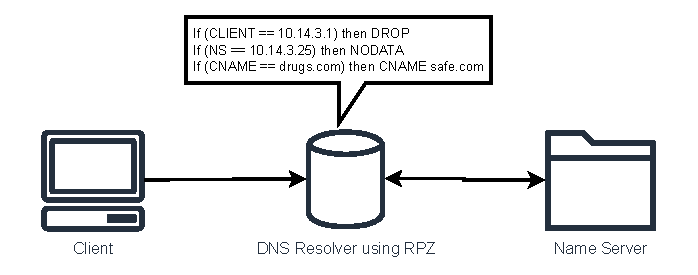
\includegraphics[width=1.0\linewidth]{figures/Response_Policy_zones.pdf}
  \caption{Un resolver DNS che sfrutta le Response Policy Zones}
  \label{fig:rpz}
\end{figure}

Le RPZ rappresentano un potente strumento per l'applicazione delle politiche di sicurezza e per proteggere la rete da attività malevole. Inoltre, il loro essere flessibili e personalizzabili, consente agli amministratori di definire policy molto specifiche, che si addatano a qualsiasi necessità. Tuttavia, per evitare falsi positivi e per mantenere l'efficacia del sistema nel tempo, le RPZ necessitano di una corretta configurazione e manutenzione. Infatti, le policy hanno costantemente bisogno di essere mantenute aggiornate, partendo da informazioni accurate ed affidabili.

Infine, si ritiene opportuno puntualizzare un limite di questa tecnologia. In particolare, le RPZ sono in grado di proteggere solamente da minaccie conosciute. Ciò deriva dalla natura stessa di questa tecnica di filtraggio, che fa affidamento su delle policy definite sulla base di minaccie necessariamente già inquadrate e studiate.

\subsubsection{Threat Intelligence Feeds}
Prima di descrivere la tecnica di filtraggio in sé, si ritiene necessario presentare brevemente i concetti ad essa associati: l'espressione \textit{cyber threat intelligence} si riferisce ad un insieme di informazioni relative a minacce informatiche potenziali o reali, utili per migliorare la situazione di un'organizzazione in termini di sicurezza.
%
Queste informazioni possono includere dettagli su tattiche, tecniche e procedure (TTP) adottate da attori malevoli noti, nonché indicatori di compromissione (IOC) come indirizzi IP, nomi di dominio e hash di malware. Nel contesto del DNS, i Threat Intelligence Feeds costituiscono dati aggiornati sui domini malevoli e relativi indirizzi IP.

I TIF possono provenire da fonti diverse, tra cui intelligence open-source, fornitori commerciali e gruppi di condivisione delle minacce specifici per settore. Questi flussi includono elenchi di IOC generati analizzando il traffico di rete, i log di sicurezza o altre fonti di intelligence. I resolver, quindi, possono utilizzare questi dati per bloccare o reindirizzare le query DNS verso domini malevoli noti.

In generale, l'integrazione dei TIF nel filtraggio DNS offre una difesa efficace contro le minacce conosciute e aiuta le organizzazioni a rilevare e prevenire gli attacchi prima che possano causare danni. Tuttavia, è importante ricordare che i flussi in questione non rappresentano una soluzione definitiva e devono essere utilizzati insieme ad altre misure di sicurezza per garantire una protezione completa.

\subsubsection{Domain Generation Algorithms}
Rappresenta una metodologia che attuano i malware per la generazione di nomi di dominio univoci, volti a consentire la comunicazione tra le vittime ed i cosiddetti server \textit{Command-and-Control} (C2). Tali domini, vengono solitamente generati partendo dalla data e ora corrente, rendendo il processo di blocco molto difficile per i  sistemi di filtraggio che si basano su liste statiche di indirizzi IP malevoli. Però, grazie a specifici algoritmi di Machine Learning, è possibile individuare questi nomi casuali, riconoscendo i pattern generati algoritmicamente. In particolare, analizzando la struttura dei domini creati dai malware, insieme al comportamento e al contesto delle query DNS, è possibile identificare e bloccare le comunicazioni con i server C2, anche se i nomi dannosi vengono utilizzati una sola volta.

\subsubsection{Uso combinato di RPZ, TIF e rilevamento DGA}
L'uso combinato di Response Policy Zones, Threat Intelligence Feeds e tecniche di rilevamento di algoritmi di generazione di domini, rappresenta un approccio promettente per migliorare l'efficacia del filtraggio DNS. Le RPZ possono intercettare le query DNS, confrontandole con blocklist e allowlist, mantenute costantemente aggiornate grazie ai TIF. A loro volta, i TIF possono integrare tecniche avanzate di rilevamento DGA per identificare domini malevoli conosciuti e sconosciuti, analizzando query anonimizzate.

Un framework che integri queste tecniche può migliorare notevolmente la capacità di rilevare e bloccare domini malevoli, minimizzando i falsi positivi e garantendo un'intelligence tempestiva e accurata. La trasparenza nel processo di filtraggio, che si concretizza nel remdere pubblicamente disponibili le liste di filtri, può favorire la fiducia degli utenti e prevenire abusi come la censura. Inoltre, il coinvolgimento della community attraverso contributi di esperti e ricercatori nell'ambito della sicureza informatica, può ulteriormente rafforzare l'efficacia del sistema.

Se da un lato ci sono dei vantaggi nel rendere pubbliche tali informazioni, dall'altro potrebbero emergere argomentazioni a sfavore di questa attività. Infatti, i malintenzionati sarebbero in grado di adattare le loro metodologie di attacco sulla base delle politiche di filtraggio facilmente consultabili. Ciononostante, questo approccio potrebbe generare dei vantaggi indiretti, derianti dal fatto che i creatori di malware sarebbero costretti a modificare i propri metodi di attacco, rendendo il loro comportamento più visibile all'interno del traffico di rete. Questo cambiamento, a sua volta, puù aiutare i ricercatori, e in generale i difensori, a venrie a conoscenza delle nuove tecniche di evasione emsse in campo dai cybercriminali \cite{DBLP:journals/corr/abs-2401-03864}.

\section{Metodologie di reingegnerizzazione software}
All'inizio degli anni '90 è emersa la forte necessità di reingegnerizzazione, alimentata soprattutto da tutti coloro che stavano migrando i sistemi informativi aziendali verso interfacce Web più moderne \cite{DBLP:conf/icse/MullerJSSTW00}. Ciò ha fatto si che il campo della reigegnerizzazione si sviluppasse per affrontare i problemi legati ai sistemi software divenuti ormai obsoleti. Tali sistemi, definiti con la parola inglese \emph{legacy}, risultavano tuttavia fondamentali per le operazioni ed i processi aziendali. Di conseguenza, da allora fino ad oggi, i ricercatori stanno lavorando per progettare dei modelli e dei piani d'azione che siano flessibili e riutilizzabili per poter essere applicati al processo di reigegnerizzazione dei software legacy \cite{Majthoub2018}.

In questa sezione verranno esaminati i concetti chiave e gli obiettivi della reingegnerizzazione, seguiti dalla descrizione di un modello generale che ne rappresenta l'architettura. Successivamente, saranno esplorati gli approcci più comuni e le fasi operative che caratterizzano questo processo. Infine, si fornirà una breve panoramica sui principali rischi associati alla reingegnerizzazione.

\subsection{Definizione e obiettivi}
Sono stati Chikofsky e Cross tra i primi ricercatori ad inquadrare la reingegnerizzazione in maniera chiara e strutturata. La loro interessante definizione descrive questo concetto come, testualmente: ``\textit{the examination and alteration of software systems to reconstitute it in new form and the subsequent implementation of the new form}'' \cite{DBLP:journals/software/ChikofskyC90}.

In termini più attuali, la reingegnerizzazione software si definisce come il processo di riprogettazione e reimplementazione di sistemi legacy con l'obiettivo di migliorarne la manutenibilità. Ciò richiede un'analisi della documentazione esistente per produrne una nuova ed equivalente, una revisione dell'architettura del sistema per riorganizzarne la struttura, e infine una reimplementazione con tecnologie o linguaggi moderni che soddisfano le esigenze attuali del mercato. Tutto questo dovrebbe essere fatto cercando di mantenere quante più funzionalità possibili del sistema rivisitato \cite{sommerville2011software}.

A differenza dell'ingegneria del software, che parte da specifiche e conduce alla creazione di un sistema attraverso design e implementazione, la reingegnerizzazione parte da un software esistente, che viene analizzato e trasformato per derivare un sistema target.

Questa distinzione non è solo teorica, ma trova applicazione concreta in una serie di situazioni che rendono la reingegnerizzazione una scelta indispensabile. Più nel detaglio, questa pratica risulta particolarmente necessaria:
\begin{itemize}
  \item quando il codice sorgente non ha più una struttura pulita e chiara, unito al fatto che la documentazione potrebbe non esistere;
  \item quando il supporto hardware e software nel sistema attuale diventa obsoleto e superato a causa di cambiamenti nelle politiche organizzative o nella competizione del mercato;
  \item quando i sistemi legacy, dopo anni di modifiche, diventano difficili ed onerosi da modificare.
\end{itemize}

\subsubsection{Obiettivi della reingegnerizzazione}
Sebbene gli obiettivi del processo di reigegnerizzazione possano variare sulla base dello scopo delle organizzazioni che lo attuano, è possibile individuarne 4 che risultano generali ed applicabili in ogni situazione \cite{rosenberg1996software}:
\begin{enumerate}
  \item \textbf{Preparazione per l'ampliamento funzionale:} la reingegnerizzazione non dovrebbe avere lo scopo diretto di migliorare le funzionalità di un sistema esistente, ma, piuttosto, di prepararlo per futuri miglioramenti. Questo include l'analisi delle attuali caratteristiche del sistema legacy per confrontarle con le specifiche desiderate, consentendo la costruzione di un sistema target più flessibile. Ad esempio, se le migliorie desiderate seguono il paradigma di programmazione oriantato agli oggetti, il sistema target può essere riprogettato utilizzando tecnologie orientate agli oggetti per semplificare il processo di incremento delle funzionalità;

  \item \textbf{Miglioramento della manutenibilità:} con il passare del tempo, i sistemi tendono a diventare sempre più complessi e costosi da mantenere a causa della struttura del codice poco chiara e della documentazione assente o obsoleta. La reingegnerizzazione mira a ridisegnare il sistema suddividendolo in moduli funzionali meglio definiti e con interfacce esplicite. Questo processo include l'aggiornamento della documentazione interna ed esterna, facilitando così gli interventi futuri;

  \item \textbf{Migrazione:} L'industria informatica è in continua evoluzione, con l'introduzione di nuove tecnologie che spesso superano e rendono obsolete quelle esistenti in tempi molto brevi. La migrazione può quindi diventare necessaria per mantenere la compatibilità con i nuovi sistemi, per sfruttare hardware e software moderni, e per evitare costi crescenti legati alla manutenzione di tecnologie superate. La reingegnerizzazione facilita questa transizione, progettando ed applicando una migrazione controllata verso nuove piattaforme hardware, sistemi operativi più moderni o linguaggi più attuali;

  \item \textbf{Miglioramento dell'affidabilità:} i sistemi legacy, nella maggior parte dei casi, non hanno mai raggiunto un livello di affidabilità particolarmente elevato. Nel tempo, le molteplici modifiche apportate a tali sistemi hanno spesso generato i cosiddetti ``effetti a catena'', ovvero situazioni in cui un intervento introduce involontariamente nuovi problemi. Per questo motivo, uno degli obiettivi principali della reingegnerizzazione è ottenere, nel sistema target, un livello di affidabilità significativamente superiore rispetto a quello del sistema originario.
\end{enumerate}

\subsection{Modello generale}
Il processo di reingegnerizzazione del software si basa su un modello generale che definisce come un sistema legacy viene trasformato in un nuovo sistema. Questo modello si articola nei tre principi fondamentali \textit{abstraction}, \textit{alteration} e \textit{refinement}, che vengono di seguito amalizzati \cite{rosenberg1996software}:
\begin{itemize}
  \item \textbf{Abstraction} si riferisce al processo di aumentare gradualmente il livello di astrazione di un sistema. Questo avviene sostituendo le informazioni dettagliate esistenti con informazioni più generali e astratte, creando una rappresentazione che enfatizza alcune caratteristiche del sistema, andando ad eliminarne altre. L'obiettivo è comprendere meglio la struttura e il funzionamento del sistema, mettendo in evidenza solo gli aspetti più rilevanti. Questo processo è parte della reverse engineering, supportata da specifici strumenti e tecniche;
  \item \textbf{Alteration} riguarda l'apportare una o più modifiche alla rappreseentazione di un sistema senza alterarne il livello di astrazione. Ad esempio, è possibile modificare il design di un componente software senza alterare i requisiti funzionali del sistema;
  \item \textbf{Refinement} è il processo inverso dell'abstraction, ovvero la discesa graduale verso un livello di astrazione più basso. Partendo da una rappresentazione astratta del sistema target, si procede verso la sua implementazione concreta, definendo dettagli sempre più specifici. Questo processo, noto come forward engineering, ricalca in parte lo sviluppo tradizionale del software, ma con alcune differenze dovute al fatto che si parte da un sistema già in essere.
\end{itemize}

Il modello generale illustra come, a seconda dell'obiettivo della reingegnerizzazione, si possa intervenire su diversi livelli di astrazione. Ad esempio, se si vuole solo tradurre il codice da un linguaggio ad un altro, non è necessaria la reverse engineering, poiché il lavoro si svolge già al livello di astrazione più basso, ovvero l'implementazione. Invece, se si vuole riprogettare l'architettura del sistema, il processo di reverse engineering diventa fondamentale e dovrebbe arrivare fino al livello dei requisiti, in modo da ricavare le caratteristiche funzionali dal design e dall'implementazione.

Nel corso di questa sezione si è fatto riferimento più volte ai concetti di reverse engineering e forward engineering, senza tuttavia approfondirne i dettagli. Di seguito, si propone una breve descrizione di queste tecniche, al fine di chiarirne il ruolo e le caratteristiche principali nel contesto della reingegnerizzazione:

\begin{itemize}
  \item Il \textbf{Reverse Engineering} è un processo fondamentale nell'ambito in questione. Il suo scopo è quello di analizzare il sistema legacy per identificarne i componenti, le loro interrelazioni e creare rappresentazioni a un livello di astrazione superiore. In pratica, si tratta di recuperare informazioni dal codice sorgente, dalla documentazione esistente e dagli esperti del sistema per comprendere appieno la struttura del software, i requisiti e il funzionamento.
  \item Il \textbf{Forward Engineering}, invece, è il processo di creazione di un nuovo sistema passando dai livelli di astrazione più alti a quelli più bassi, andando a sostituire gradualmente le informazioni astratte con dettagli più specifici. Questo movimento verso il basso corrisponde al normale ciclo di sviluppo software, che passa dai requisiti al design, fino ad arrivare all'implementazione fisica del sistema.
\end{itemize}

\subsection{Approcci e fasi del processo}
Esistono tre doversi approcci alla reingegnerizzazione del software, i quali si differenziano per la quantità e la velocità con cui il sistema legacy viene sostituito con il sistema target. Ogni approccio è caratterizzato da vantaggi e rischi specifici, che vengono ora discussi nel dettaglio \cite{Majthoub2018,rosenberg1996software}:
\begin{enumerate}
  \item \textbf{Big Bang}: questo approccio prevede la sostituzione dell'intero sistema in un unico momento, e di solito viene messo in campo per affrontare problemi immediati come una migrazione di architettura. Il vantaggio principale è che il sistema viene trasferito in un nuovo ambiente senza dover sviluppare interfacce tra i componenti vecchi e nuovi. Lo svantaggio, però, è che il risultato finale tende ad essere un progetto monolitico, caratteristica non sempre adeguata, soprattutto per i sistemi di grandi dimensioni. Inoltre, le modifiche apportate al sistema vecchio durante la transizione devono essere integrate nel nuovo, rendendo difficile mantenere l'allineamento e preservare tutte le funzionalità esistenti. In più, il rischio di questo approccio risulta elevato in quanto il nuovo sistema deve essere funzionalmente intatto e operare in parallelo con quello vecchio fino alla completa sostituzione;

  \item \textbf{Incrementale}: l'approccio in questione prevede la reingegnerizzazione graduale di sezioni del sistema, che vengono integrate in nuove versioni quando sopraggiunge la necessità per soddisfare nuovi obiettivi. Questo metodo suddivide il progetto in porzioni più contenute basate sulla struttura esistente del sistema, permettendo così uno sviluppo più rapido delle componenti e una maggiore facilità nel tracciare gli errori. Inoltre, gli stakeholders possono monitorare i progressi attraverso le versioni intermedie e segnalare tempestivamente eventuali funzionalità mancanti o problemi individuati. Tuttavia, questo approccio richiede tempi più lunghi per il completamento del sistema, dato che le versioni intermedie necessitano di un controllo accurato della configurazione. Inoltre, non permette una completa ristrutturazione dell'architettura, limitandosi alle modifiche interne delle sezioni reingegnerizzate. Nonostante ciò, il rischio complessivo è inferiore rispetto all'approccio ``Big Bang'', poiché i rischi legati a ciascuna componente possono essere gestiti e monitorati separatamente;

  \item \textbf{Evolutivo}: l'approccio ``Evolutivo'' prevede la sostituzione graduale delle sezioni del sistema originale con parti reingegnerizzate, selezionate in base alla loro funzionalità piuttosto che alla struttura del sistema esistente (come avviene nell'approccio ``Incrementale''). Il sistema target viene costruito utilizzando moduli coesi dal punto di vista funzionale, riorganizzando le componenti attuali per funzioni specifiche. Tra i vantaggi principali vi sono un design modulare che facilita la manutenzione e un focus su unità funzionali più semplici, che rende particolarmente agevole l'adozione di tecnologie orientate agli oggetti. Tuttavia, questo approccio richiede un'attenta identificazione delle funzioni simili, spesso distribuite nel sistema originale, e può introdurre difficoltà di integrazione tra le componenti, con possibili peggioramenti delle prestazioni dovuti alla reingegnerizzazione isolata delle sezioni funzionali.
\end{enumerate}

Dopo aver analizzato i principali approcci adottati nella reingegnerizzazione, è importante approfondire le fasi fondamentali che guidano la trasformazione del sistema legacy in un nuovo sistema. Queste fasi, articolate in cinque passaggi chiave, hanno compiti specifici volti a garantire una transizione efficace verso il sistema target \cite{rosenberg1996software}:
\begin{enumerate}
  \item \textbf{Formazione del team di reingegnerizzazione}: il team guiderà l'intero processo, richiedendo una formazione approfondita sulla gestione del cambiamento tecnologico, sui principi della reingegnerizzazione e sui processi di sviluppo del sistema target. Le loro attività comprenderanno la definizione di obiettivi, strategie e piani d’azione, oltre all'identificazione e all'acquisto di strumenti adeguati. Sarà loro compito promuovere il progetto all’interno dell’organizzazione, offrire supporto al personale e garantire l’applicazione corretta del processo. Infine, saranno essenziali buone capacità relazionali per affrontare eventuali resistenze al cambiamento;

  \item \textbf{Analisi di fattibilità del progetto}: il primo compito del team di reingegnerizzazione è valutare i bisogni organizzativi e gli obiettivi soddisfatti dal sistema esistente, garantendo che la strategia sia allineata alle esigenze aziendali. È fondamentale analizzare il software attuale per identificare problemi, scopi e vincoli, stimando il ritorno sull’investimento. Gli obiettivi, come il miglioramento delle prestazioni o la riduzione dei costi, devono essere misurabili e confrontati con i costi della reingegnerizzazione e il valore aggiunto previsto;

  \item \textbf{Analisi e pianificazione}: questa fase si articola in tre passaggi principali: l'analisi del sistema legacy, la definizione delle caratteristiche del sistema target e la creazione di un ambiente di test. L'analisi inizia con la raccolta e lo studio del codice e della documentazione disponibili, al fine di identificare peculiarità e problemi di qualità del software esistente. Successivamente, vengono definite le modifiche richieste, come la piattaforma hardware, il sistema operativo, la struttura del design e il linguaggio. Infine, si sviluppa un ambiente di test standard, necessario per garantire l’equivalenza funzionale tra il nuovo sistema e quello originale, assicurando la tracciabilità delle funzioni esistenti;

  \item \textbf{Implementazione della reingegnerizzazione}: dopo che sono stati definiti gli obiettivi e l'approccio, e dopo aver analizzato il sistema legacy, iniziano le fasi di reverse e forward engineering. La prima scompone le funzioni del sistema legacy fino a raggiungere il livello di astrazione desiderato, utilizzando strumenti che siano compatibili con gli obiettivi. In seguito, la seconda riprende dal livello raggiunto per sviluppare il nuovo design, seguendo il normale processo di sviluppo software. Durante questa fase, è fondamentale evitare modifiche o aumenti di funzionalità per semplificare la validazione, applicando tecniche per il controllo della qualità, e monitorando continuamente i miglioramenti e i potenziali rischi;

  \item \textbf{Test e transizione}: man mano che le funzionalità del nuovo sistema aumentano, è necessario effettuare test per individuare eventuali errori introdotti durante la reingegnerizzazione. Le tecniche di testing sono le stesse utilizzate per lo sviluppo di un sistema da zero. Se i requisiti del nuovo sistema coincidono con quelli del sistema legacy, è possibile riutilizzare i test e l'ambiente sviluppati durante la fase di pianificazione, confrontando i risultati per verificare la funzionalità del sistema target. Inoltre, la documentazione del sistema legacy deve essere aggiornata o sostituita per riflettere il nuovo sistema e fornire le informazioni necessarie per la sua gestione e manutenzione.
\end{enumerate}

Seguire queste fasi in modo strutturato è cruciale per garantire il successo di un progetto di reingegnerizzazione del software, riducendo i rischi e ottimizzando l'utilizzo di tempo e risorse.

\subsection{Panoramica sui rischi}
Per concludere la sezione corrente e fornire un quadro ancora più completo sulla reingegnerizzazione, si ritiene opportuno fare una breve panoramica sui potenziali rischi che questo importante processo si porta dietro, soprattutto se non viene gestito in maniera appropriata.

La reingegnerizzazione del software, pur offrendo vantaggi significativi, comporta rischi che devono essere identificati e gestiti con attenzione per garantire il successo del progetto. Questi rischi si manifestano in diverse aree chiave, tra cui il processo, il reverse engineering, il forward engineering, il personale, gli strumenti e la strategia \cite{rosenberg1996software}.
\begin{itemize}
  \item Un rischio rilevante riguarda l'elevato costo del \textbf{processo} di reingegnerizzazione manuale, che potrebbe non garantire benefici proporzionati nei tempi previsti. Inoltre, la mancanza di supporto da parte del management o una selezione inadeguata dei sottosistemi da reingegnerizzare possono compromettere il progetto. Altri rischi includono una gestione insufficiente della configurazione, l'assenza del controllo qualità o di un programma di metriche adeguato, e la carenza di esperti con conoscenze sugli applicativi locali.
  \item Nel \textbf{reverse engineering}, una delle principali difficoltà è il recupero di requisiti e informazioni di progettazione dal codice sorgente, specialmente se il linguaggio utilizzato non consente una rappresentazione astratta efficace. La perdita di informazioni aziendali incorporate nel codice costituisce un ulteriore rischio critico.
  \item Anche il \textbf{forward engineering} presenta sfide significative. L'introduzione di nuovi requisiti o funzionalità può complicare il processo di validazione, mentre la migrazione dei dati esistenti e una preparazione insufficiente durante il reverse engineering possono influire negativamente sull'esito del progetto.
  \item I principali rischi legati al \textbf{personale} riguardano la mancanza di competenze adeguate nella reingegnerizzazione e la scarsa esperienza, che possono influire negativamente sull'efficacia del progetto. Inoltre, i programmatori potrebbero lavorare in modo volutamente meno efficiente per ostacolare un'iniziativa percepita come impopolare.
  \item Le problematiche connesse agli \textbf{strumenti} includono la dipendenza da soluzioni che non funzionano come previsto o che risultano nuove e immature. Anche la stabilità dei fornitori e la qualità complessiva degli strumenti possono rappresentare un rischio significativo.
  \item  I rischi \textbf{strategici} includono l'impegno prematuro in una soluzione di reingegnerizzazione per l'intero sistema, la mancanza di una visione a lungo termine e l'adozione di obiettivi irrealistici o poco solidi. Altri problemi possono derivare dalla scelta di approcci che non rispettano gli scopi aziendali, i limiti di budget o le scadenze, oltre che dall'assenza di un piano per l'utilizzo degli strumenti di reingegnerizzazione.
\end{itemize}
